Nuance image loaded by the function \texttt{load\_nuance\_image} in Code \ref{code:load-nuance} is saved in the ENVI format.
The spectral image is saved as a raw file with the BIL interleave. 

Preview by FreeLook software is shown in Figure \ref{fig:nuance-preview}.

\begin{figure}[H]
    \centering
    \caption{Preview of the Nuance image in FreeLook software}
    \label{fig:nuance-preview}
    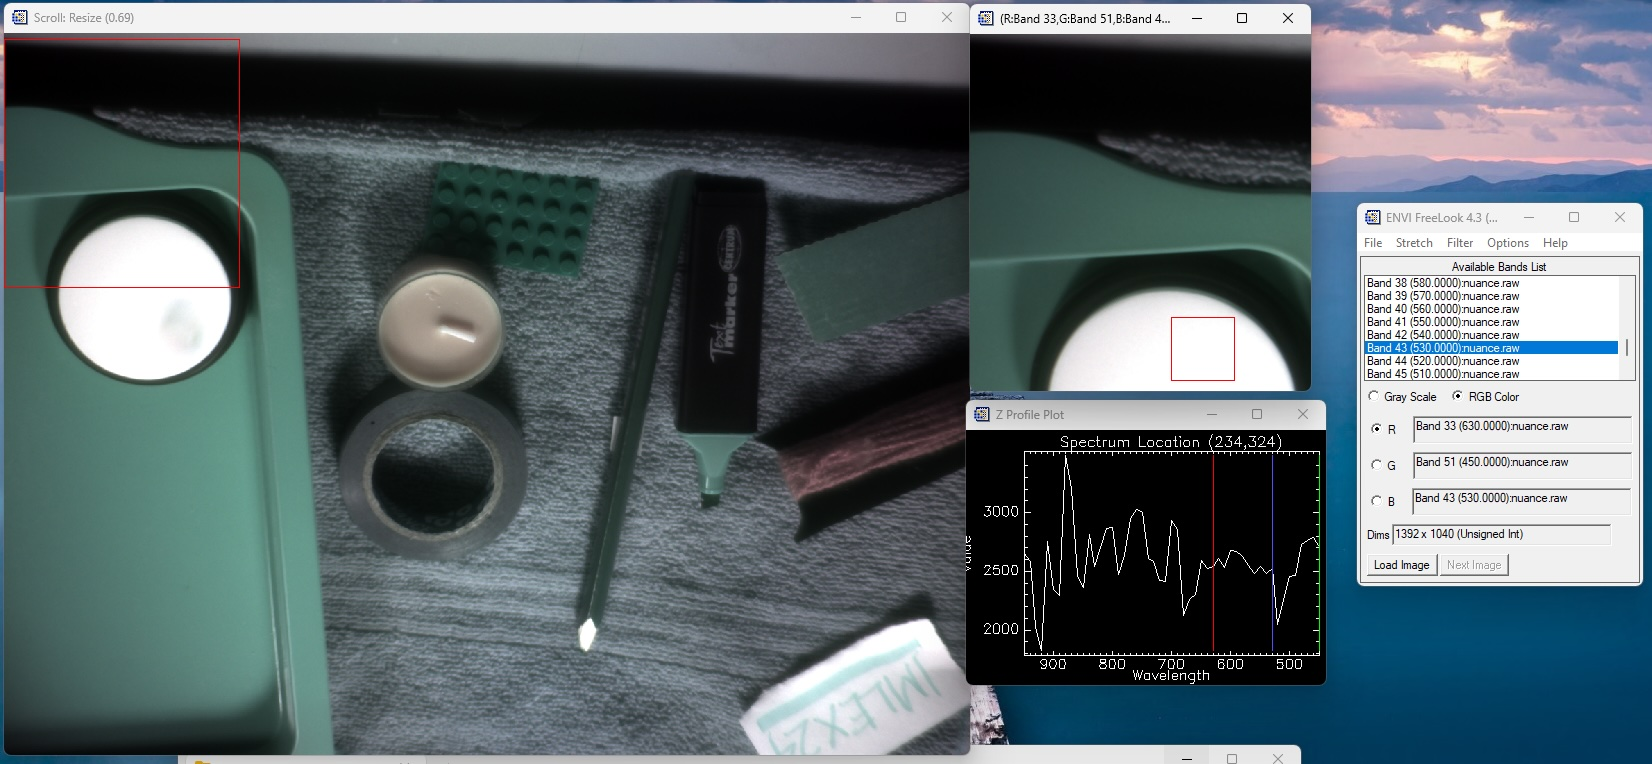
\includegraphics[width=0.5\textwidth]{./fig-task2/nuance.jpg}
\end{figure}


The header file is shown in Code \ref{code:nuance-hdr}.

\begin{lstlisting}[caption=Saved ENVI header file, label={code:nuance-hdr}]
ENVI
ENVI description = {File Imported into ENVI}
file type = ENVI
lines = 1040
samples = 1392
bands = 51
interleave = bil
data type = 12
header offset = 0
byte order = 0
wavelength = {
    950.0,
    ...,
    460.0,
    450.0
}

\end{lstlisting}